%!TEX root = edance.tex
%%%%%%%%%%%%%%%%
%  CHAPTER 10  %
%%%%%%%%%%%%%%%%
\chapter{Complete MOS Small-Signal Model}
\label{ch:ch10_mos_ss_ac}
\graphicspath{{./figures/figs_ch10_mos_ss_ac/}}
%%%%%%%%%%%%%%%%%%%%%%%%%%%%%%%%%%%%%%%%%%%%%%%%%%%%%%%%%%%%%%%%%%%%%%%%%%%%%%%%%%%%%%%%
%%%%%%%%%%%%%%%%%%%%%%%%%%%%%%%%%%%%%%%%%%%%%%%%%%%%%%%%%%%%%%%%%%%%%%%%%%%%%%%%%%%%%%%%
%                                   SECTION 10.1                                       %
%%%%%%%%%%%%%%%%%%%%%%%%%%%%%%%%%%%%%%%%%%%%%%%%%%%%%%%%%%%%%%%%%%%%%%%%%%%%%%%%%%%%%%%%
%%%%%%%%%%%%%%%%%%%%%%%%%%%%%%%%%%%%%%%%%%%%%%%%%%%%%%%%%%%%%%%%%%%%%%%%%%%%%%%%%%%%%%%%
\section{Chapter Preview}
In this chapter we make amends for ignoring charge storage effects in the MOS transistor.  In particular, we focus on the MOSFET capacitance in the saturation regime, including the Gate-Source $C_{gs}$, Gate-drain $C_{gd}$, and drain/source to bulk $C_{db}$ and $C_{sb}$.  This will result in a complete \emph{four terminal} MOS small-signal model.

Some of these capacitances are parasitic to the MOSFET, and they introduce undesirable poles and zeros to the circuit.  This has the negative effect of limiting the bandwidth, and slowing the circuit down.

A more subtle effect comes from the so-called "Back-Gate Effect", or how the threshold voltage can be modulated by a source-body bias.  We will model this in the small-signal AC circuit by introducing a back-gate transconductance.  This will result in the complete \emph{four terminal} MOS small-signal model.  This model will be used extensively throughout the rest of this book.
%
%\subsection{What we’ve ignored…until now!}
%
%\begin{figure}[tb]
%\centering
%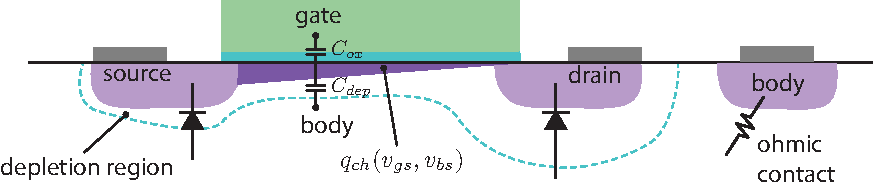
\includegraphics[width=.75\columnwidth]{mos_backgate}
%\caption{mos backgate} \label{fig:}
%\end{figure}
%
% The fourth terminal of the MOSFET is the body of the transistor
% The junctions of the transistor form $PN$-junction diodes,and naturally this introduces parasitic capacitance from source and drain to the body or bulk.
% Notice that while the source/drain form reverse-biased (nominally) junctions with the body, the body contact is "ohmic" meaning that the body is controlled direction by the voltage on the body terminal.
% The inversion charge is therefore modulated by the body terminal, which acts like a "back gate".
% 
%%%%%%%%%%%%%%%%%%%%%%%%%%%%%%%%%%%%%%%%%%%%
%                 FIGURE                   %
%%%%%%%%%%%%%%%%%%%%%%%%%%%%%%%%%%%%%%%%%%%%
% \begin{figure}[H]
% \centering
% \includegraphics[scale=1.00]{null}
% \caption{null}
% \label{fig:ch10_intro}
% \end{figure}
%%%%%%%%%%%%%%%%%%%%%%%%%%%%%%%%%%%%%%%%%%%%
\newpage
%%%%%%%%%%%%%%%%%%%%%%%%%%%%%%%%%%%%%%%%%%%%
%                 FIGURE                   %
%%%%%%%%%%%%%%%%%%%%%%%%%%%%%%%%%%%%%%%%%%%%
\begin{figure}[t]
\centering
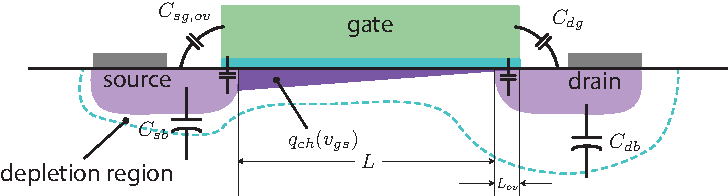
\includegraphics[width=\columnwidth]{mos_caps_xsect}
\caption{Cross section of an MOS transistor highlighting the internal capacitance arising from $q_{ch}$ and the parasitic capacitors due to $PN$-junctions, overlap and fringing capacitance.}
\label{fig:moscapsxsect}
\end{figure}
%%%%%%%%%%%%%%%%%%%%%%%%%%%%%%%%%%%%%%%%%%%%%%%%%%%%%%%%%%%%%%%%%%%%%%%%%%%%%%%%%%%%%%%%
%%%%%%%%%%%%%%%%%%%%%%%%%%%%%%%%%%%%%%%%%%%%%%%%%%%%%%%%%%%%%%%%%%%%%%%%%%%%%%%%%%%%%%%%
%                                   SECTION 10.2                                       %
%%%%%%%%%%%%%%%%%%%%%%%%%%%%%%%%%%%%%%%%%%%%%%%%%%%%%%%%%%%%%%%%%%%%%%%%%%%%%%%%%%%%%%%%
%%%%%%%%%%%%%%%%%%%%%%%%%%%%%%%%%%%%%%%%%%%%%%%%%%%%%%%%%%%%%%%%%%%%%%%%%%%%%%%%%%%%%%%%
\section{MOSFET Capacitance in Saturation}
%%%%%%%%%%%%%%%%%%%%%%%%%%%%%%%%%%%%%%%%%%%%
%             SUBSECTION 10.2.1            %
%%%%%%%%%%%%%%%%%%%%%%%%%%%%%%%%%%%%%%%%%%%%
\subsection{MOSFET Cross Section}
As shown in the device cross-section of \emph{Fig.~\ref{fig:moscapsxsect}}, MOSFETs have many capacitances\index{MOSFET!capacitances}. Some are critical to the function of the MOS, such as $C_{ox}$.  However, others are undesired parasitics\index{Parasitic capacitance}.  Let's analyze where each capacitance comes from step-by-step.  For now we will ignore the influence of the back gate, and just assume that the body is AC grounded. In this case, note that channel charge is mostly controlled by gate-source voltage and not the drain voltage.  
%%%%%%%%%%%%%%%%%%%%%%%%%%%%%%%%%%%%%%%%%%%%
%             SUBSECTION 10.2.2            %
%%%%%%%%%%%%%%%%%%%%%%%%%%%%%%%%%%%%%%%%%%%%
\subsection{Gate-Source Capacitance \texorpdfstring{$C_{GS}$}{}}
Since the drain is isolated from the channel (in saturation), the oxide capacitance $C_{ox}$ is formed from the gate to source, as shown in \emph{Fig.~\ref{fig:mos_caps_Cgs}}.  But since the inversion charge is "wedge" shaped (inversion decreases as we travel from the source to drain), the \textbf{effective capacitance}\index{MOSFET!capacitances!gate-source} is lower.  A detailed calculation shows that:
    \begin{align}
        \Aboxed{C_{gs} &= \left(\frac{2}{3}\right)W\,L\,C_{ox} + C_{ov}} &\textit{Gate-source capacitance in saturation}
    \end{align} 
We include a \textbf{parasitic overlap capacitance}\index{MOSFET!parasitic overlap capacitance} $C_{ov}$ along source edge of gate:
    \begin{align}
        \Aboxed{C_{ov} &= L_{ov}\,W\,C_{ox}} &\textit{MOSFET parasitic overlap capacitance}
    \end{align}
The physical origin of the overlap capacitance is the overlap between the gate and the source, resulting from imperfect alignment between the gate and the source.  This causes a diffusion region to grow under the gate.   In a "good" transistor, $L_{ov} \ll L$, so $C_{gd} \ll C_{gs}$.  The actual value is higher due to fringing fields that leak from the gate to the top of the source and drain junctions.
%%%%%%%%%%%%%%%%%%%%%%%%%%%%%%%%%%%%%%%%%%%%
%                 FIGURE                   %
%%%%%%%%%%%%%%%%%%%%%%%%%%%%%%%%%%%%%%%%%%%%
\begin{figure}[H]
\centering
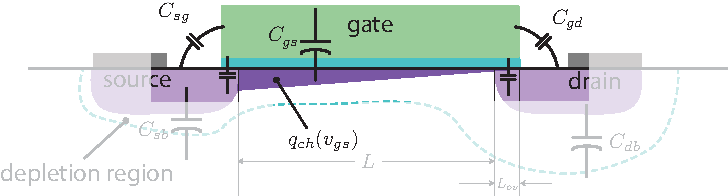
\includegraphics[width=\columnwidth]{mos_caps_Cgs}
\caption{The gate-source capacitance is made of two parts; the inversion charge $q_{ch}(v_{gs})$ which is part of the MOS-C internal structure and depends on $C_{ox}$, and other parasitic capacitors.} \label{fig:mos_caps_Cgs}
\end{figure}
%%%%%%%%%%%%%%%%%%%%%%%%%%%%%%%%%%%%%%%%%%%%
\newpage
%%%%%%%%%%%%%%%%%%%%%%%%%%%%%%%%%%%%%%%%%%%%
%                 FIGURE                   %
%%%%%%%%%%%%%%%%%%%%%%%%%%%%%%%%%%%%%%%%%%%%
\begin{figure}[t]
\centering
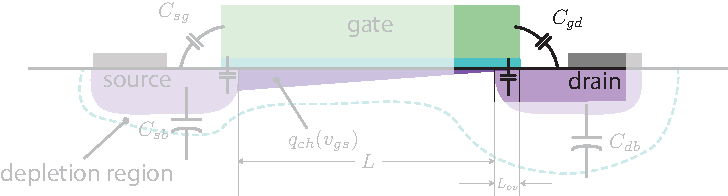
\includegraphics[width=\columnwidth]{mos_caps_Cgd}
\caption{The gate-drain capacitance is a parasitic capacitance due to oxide/drain diffusion overlap and fringing terms shown.}
\label{fig:mos_caps_Cgd}
\end{figure}
%%%%%%%%%%%%%%%%%%%%%%%%%%%%%%%%%%%%%%%%%%%%
%             SUBSECTION 10.2.3            %
%%%%%%%%%%%%%%%%%%%%%%%%%%%%%%%%%%%%%%%%%%%%
\subsection{Gate-Drain Capacitance \texorpdfstring{$C_{GD}$}{}}
Focusing now on the drain side, \emph{Fig.~\ref{fig:mos_caps_Cgd}}, we see that the same overlap occurs on the drain side.  This \textbf{gate-drain capacitance}\index{MOSFET!capacitances!gate-drain} in another undesirable parasitic:
    \begin{align}
        \Aboxed{C_{gd} &= C_{ov} + C_{fringe} = L_{ov}\,W\,C_{ox} + C_{fringe}} &\textit{Gate-drain capacitance in saturation}
    \end{align}
Since the MOSFET drain and source are physically identical, this is not surprising.\footnote{Some special devices use asymmetric source/drain junctions.}  Just keep in mind that this capacitance is not due to change in inversion charge in channel.
%%%%%%%%%%%%%%%%%%%%%%%%%%%%%%%%%%%%%%%%%%%%
%             SUBSECTION 10.2.4            %
%%%%%%%%%%%%%%%%%%%%%%%%%%%%%%%%%%%%%%%%%%%%
\subsection{Drain/Source-Bulk Capacitances \texorpdfstring{$C_{DB}\text{ and }C_{SB}$}{}}
The \textbf{Drain-Bulk}\index{MOSFET!capacitances!drain-bulk} and \textbf{Source-Bulk}\index{MOSFET!capacitances!source-bulk} capacitances are two more undesired parasitics.  They are caused by $PN$-junction depletion regions that isolate the drain/source from the body. The junction forms a "box" inside the body, and so there are five junctions to consider. \textit{Four side-wall junctions} and one \textit{bottom wall} junction, shown in \emph{Fig.~\ref{fig:cap_junc_3d}}.
%%%%%%%%%%%%%%%%%%%%%%%%%%%%%%%%%%%%%%%%%%%%
%                 FIGURE                   %
%%%%%%%%%%%%%%%%%%%%%%%%%%%%%%%%%%%%%%%%%%%%
\begin{figure}[H]
\centering
\subcaptionbox{\label{fig:cap_junc_3d}}{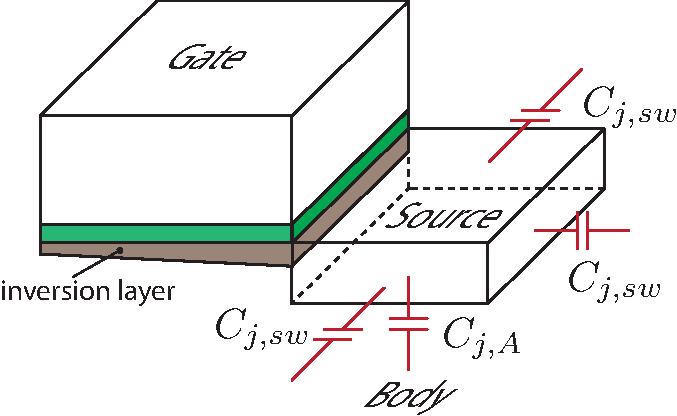
\includegraphics[width=.6\columnwidth]{cap_junc_3d}}
\hspace{0.75cm}
\subcaptionbox{\label{fig:mos_layout_top}}{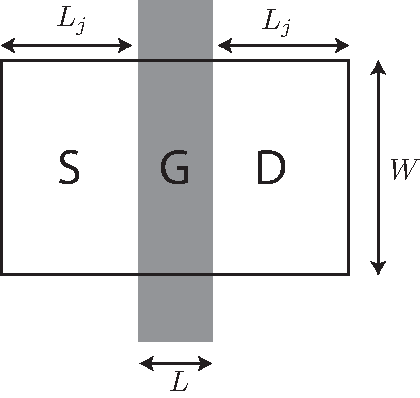
\includegraphics[width=.3\columnwidth]{mos_layout_top}}
\caption{(a) The drain/source junctions form $PN$-junctions with the body.  Under normal operating conditions, these capacitors are reverse biased.  There are "sidewall" contributions $C_{j,sw}$ shown and a bottom plate term $C_{j,A}$.  (b)  The junction perimeter and area is calculated from the MOS layout and depends on the width $W$ of the device in addition to the length of the junctions $L_j$.} 
\end{figure}
%%%%%%%%%%%%%%%%%%%%%%%%%%%%%%%%%%%%%%%%%%%%
\newpage
The capacitance is defined in terms of the junction areas $A_{s,j}$ and $A_{d,j}$ and the junction perimeters, $P_{s,j}$ and $P_{d,j}$.  As shown in  \emph{Fig.~\ref{fig:mos_layout_top}}, besides the transistor $L$ and $W$ parameters, we need to know the length of the source and drain diffusion regions, $L_j$, to calculate the area and perimeter.  The junction area is simply $L_j \cdot W$ whereas the perimeter is $(2\cdot L_j + W)$, because the inner junction facing the channel is isolated from the bulk.
    \begin{align}
        \Aboxed{C_{sb} &= \left( \frac{C_{j_0}}{\sqrt{ 1 + V_{SB}/|\phi_{p}|}} \right)A_{s,j}
                    + \left( \frac{C_{{j,sw}_0}}{\sqrt{ 1 + V_{SB}/|\phi_p|}} \right)P_{s,j}}
        & \textit{Source-body capacitance}
    \end{align}
    \begin{align}
        \Aboxed{C_{db} &= \left( \frac{C_{j_0}}{\sqrt{ 1 + V_{DB}/|\phi_{p}|}}\right)A_{d,j}
                    + \left( \frac{C_{{j,sw}_0}}{\sqrt{ 1 + V_{DB}/|\phi_p|}} \right)P_{d,j}}
        & \textit{Drain-body capacitance}
    \end{align}
Although we have used a \textbf{grading coefficient}\index{MOSFET!capacitance grading coefficient} of $1/2$ for junctions (leading to square roots in the denominator), in reality this is a parameter that you will adjust based on process parameters.

It is important to realize that the source/drain are symmetric.  The source/drain is defined by potentials/biasing and the schematic rather than the process. For this reason, the doping parameters for the source and drain are symmetric, and so the calculations for the source and drain to bulk are very much the same.  Of course, the area of the junctions may differ based on the device layout.	Some special technologies (high breakdown devices) have an asymmetric source/drain, but this is rare.

\textit{If the source and body are both AC grounded, then the source-to-bulk capacitance does not play a role in AC response, and it is excluded from the model.}
%%%%%%%%%%%%%%%%%%%%%%%%%%%%%%%%%%%%%%%%%%%%
%             SUBSECTION 10.2.5            %
%%%%%%%%%%%%%%%%%%%%%%%%%%%%%%%%%%%%%%%%%%%%
\subsection{Three Terminal Small Signal Model Including Capacitors}
We can now update our three-terminal small-signal model to include three capacitors, as shown in \emph{Fig.~\ref{fig:mos3term_ac}}.  The capacitance $C_{gs}$ is a combination of the gate-oxide capacitance (recall the factor of $2/3$ arising from the uneven charge distribution in the saturation region), and any overlap and fringing capacitance between the gate and the source.  On the other hand, the capacitance $C_{gd}$ is all due to overlap, because in the saturation region the drain is isolated from the channel due to pinch-off.  The capacitance $C_{db}$ simply accounts for the reverse-biased $PN$-junction capacitance from the drain diffusion region to the body of the transistor.  The capacitor $C_{sb}$ is missing from the model, because it is shorted out in the three terminal model if we assume the source/bulk are tied together.  In practice, this may not be true and we should include this capacitor as well.  We will cover this in the full four-terminal model.
%%%%%%%%%%%%%%%%%%%%%%%%%%%%%%%%%%%%%%%%%%%%
%                 FIGURE                   %
%%%%%%%%%%%%%%%%%%%%%%%%%%%%%%%%%%%%%%%%%%%%
\begin{figure}[H]
\centering
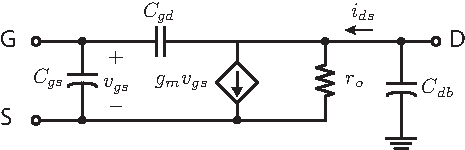
\includegraphics[scale=1.35]{mos3term_ac}
\caption{The complete three terminal model of a MOSFET with source-body tied together includes  capacitance $C_{gs}$ and the parasitic $C_{gd}$ and $C_{db}$.}
\label{fig:mos3term_ac}
\end{figure}
%%%%%%%%%%%%%%%%%%%%%%%%%%%%%%%%%%%%%%%%%%%%
\newpage
%%%%%%%%%%%%%%%%%%%%%%%%%%%%%%%%%%%%%%%%%%%%
%                 FIGURE                   %
%%%%%%%%%%%%%%%%%%%%%%%%%%%%%%%%%%%%%%%%%%%%
\begin{figure}[t]
\centering
\subcaptionbox{\label{fig:mos4term}}{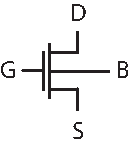
\includegraphics[width=.15\columnwidth]{mos4term}}
\subcaptionbox{\label{fig:mos_backgate}}{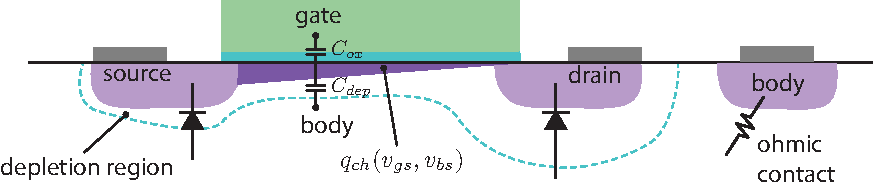
\includegraphics[width=.95\columnwidth]{mos_backgate}}
\caption{(a) The body terminal of a MOSFET is an independent fourth terminal of the device.  (b) Variations in the body voltage couple into the channel charge through $C_{dep}$, in a similar manner as gate voltage variations couple into the channel charge through $C_{gs}$.} 
\end{figure}
%%%%%%%%%%%%%%%%%%%%%%%%%%%%%%%%%%%%%%%%%%%%%%%%%%%%%%%%%%%%%%%%%%%%%%%%%%%%%%%%%%%%%%%%
%%%%%%%%%%%%%%%%%%%%%%%%%%%%%%%%%%%%%%%%%%%%%%%%%%%%%%%%%%%%%%%%%%%%%%%%%%%%%%%%%%%%%%%%
%                                   SECTION 10.3                                       %
%%%%%%%%%%%%%%%%%%%%%%%%%%%%%%%%%%%%%%%%%%%%%%%%%%%%%%%%%%%%%%%%%%%%%%%%%%%%%%%%%%%%%%%%
%%%%%%%%%%%%%%%%%%%%%%%%%%%%%%%%%%%%%%%%%%%%%%%%%%%%%%%%%%%%%%%%%%%%%%%%%%%%%%%%%%%%%%%%
\section{Back-Gate Effect}
%%%%%%%%%%%%%%%%%%%%%%%%%%%%%%%%%%%%%%%%%%%%
%             SUBSECTION 10.3.1            %
%%%%%%%%%%%%%%%%%%%%%%%%%%%%%%%%%%%%%%%%%%%%
\subsection{All MOSFETS have a "Back Door"}
So far we have been ignoring the body terminal of the device, shown explicitly in \emph{Fig.~\ref{fig:mos4term}}.  The MOS transistor has some symmetry that you should appreciate between the source and drain.  It is less obvious, but there is a symmetry between the gate and the body if you think about how the inversion charge depends on both voltages. We will show that the body can act like a "back gate", and control the inversion and thus the current in the device, as shown in \emph{Fig.~\ref{fig:mos_backgate}}.  It is something we have ignored, because in many instances the body terminal is simply tied to the source, and the source is sometimes at ground or $V_{SS}$ for NMOS, or supply or $V_{DD}$ for PMOS.  What we would like to understand is what happens if there is a DC voltage or an AC voltage swing on the body terminal.
%%%%%%%%%%%%%%%%%%%%%%%%%%%%%%%%%%%%%%%%%%%%
%             SUBSECTION 10.3.2            %
%%%%%%%%%%%%%%%%%%%%%%%%%%%%%%%%%%%%%%%%%%%%
\subsection{Body Bias Affects: \texorpdfstring{$V_T$}{Threshold Voltage} - DC Signals}
From our calculations of the MOS capacitor, we know that the body bias $V_{SB}$ has an impact on the channel charge.  There is a depletion capacitance between the transistor body and the channel:
    \begin{equation}
        C_{dep} = \mathlarger{\frac{\varepsilon_s}{x_{dep,MAX}}}
    \end{equation}
If we take into account the body voltage with respect to the source, the amount of inversion charge is given by:
    \begin{equation}
        Q_{inv} =  -C_{ox}(V_{GS} - V_T) - C_{dep}V_{BS}
    \end{equation}
Here the role of the back-gate is shown explicitly and symmetrically with respect to the front gate.  Whereas the front gate, or simply the gate, affects the inversion charge through $C_{ox}$, the back-gate affects the amount of inversion charge through $C_{dep}$.  Let's factor out $C_{ox}$ and note that $V_{SB} = - V_{BS}$:
    \begin{equation}
        Q_{inv} =  -C_{ox}\left[ {V_{GS} - V_T + \left( \frac{C_{dep}}{C_{ox}} \right)V_{SB}} \right]
    \end{equation}
Written in this form, we can lump the back-gate effect into a change in the threshold voltage:
    \begin{equation}
        V_T(V_{SB}) = V_{T_0} + \left( \frac{C_{dep}}{C_{ox}} \right)V_{SB}
        \label{eq:charge_back_gate}
    \end{equation}
In \emph{Eq.~\ref{eq:charge_back_gate}}, $V_{T_0}$ is the zero $V_{SB}$ threshold voltage:
    \begin{equation}
        V_{T_0} = V_T(0) = V_{FB} - 2\,\phi_p + \frac{1}{C_{ox}} \sqrt{2\,q\,\varepsilon_s\,N_A(-2\,\phi_p)}
    \end{equation}
The change in threshold due to body bias is given by:
    \begin{equation}
        \Delta V_T = \frac{1}{C_{ox}} \sqrt{2\,q\,\varepsilon_s\,N_A} \left(\sqrt{-2\,\phi_p + V_{SB}} - \sqrt{-2\,\phi_p} \right)
        = \gamma \left( {\sqrt{V_{SB} - 2\,\phi_p} - \sqrt{-2\,\phi_p}} \right)
    \end{equation}
This is written more compactly in the following form:
    \begin{align}
        \Aboxed{V_T &= V_{T_0} + \gamma \left( \sqrt{V_{SB} - 2\,\phi_p} - \sqrt{-2\,\phi_p} \right)} &\textit{Threshold voltage with body bias}
        \label{eq:vtbias}
    \end{align}
$\gamma$ is a \textbf{device parameter}\index{MOSFET!device parameter} in \emph{Eq.~\ref{eq:vtbias}}:
    \begin{align}
        \Aboxed{\gamma &= \frac{\sqrt{2\,q\,\varepsilon_s\,N_A}}{C_{ox}}} &\textit{MOSFET device parameter}
    \end{align}
%%%%%%%%%%%%%%%%%%%%%%%%%%%%%%%%%%%%%%%%%%%%
%             SUBSECTION 10.3.3            %
%%%%%%%%%%%%%%%%%%%%%%%%%%%%%%%%%%%%%%%%%%%%
\subsection{Role of the Substrate Potential - AC Signals}
Since $V_{SB}$ changes the threshold voltage, which in turn changes the drain current, the body acts like a "back-gate", and it should cause an AC current to flow in response to an AC signal between the body and source.  The \textbf{back-gate transconductance}\index{MOSFET!back-gate transconductance} is defined as:
    \begin{equation} 
        g_{mb} = \frac{\Delta i_D}{\Delta v_{BS}} \bigg\rvert_Q
        = \frac{\partial i_D}{\partial v_{BS}} \bigg\rvert_Q
    \end{equation}
We can simplify this calculation by using the chain rule and taking advantage of our previous calculation of the change in $V_T$:
    \begin{equation}
        g_{mb} = \frac{\partial I_D}{\partial V_{BS}} \bigg\rvert_Q
        = \frac{\partial I_D}{\partial V_{T}} \bigg\rvert_Q \cdot \frac{\partial V_{T}}{\partial V_{BS}} \bigg\rvert_Q
    \end{equation}
The threshold voltage is given by \emph{Eq.~\ref{eq:vtbias}}.  Taking the derivatives with $V_{BS}$ and $V_T$ results in the following:
    \begin{equation}
        g_{mb} = \frac{\partial I_D}{\partial V_{BS}} \bigg\rvert_Q
        = \frac{\partial I_D}{\partial V_{T}} \bigg\rvert_Q \cdot \frac{\partial V_{T}}{\partial V_{BS}} \bigg\rvert_Q
        = \frac{\gamma\,g_m}{2\sqrt{-V_{BS} - 2\,\phi_p}}
    \end{equation}
You can also intuitively guess that the answer should in fact be equal to:
    \begin{align}
        \Aboxed{g_{mb} &= g_m \left(\frac{C_{dep}}{C_{ox}} \right)} &\textit{Back-gate transconductance}
    \end{align}
In most transistors $C_{ox} > C_{dep}$, so the back-gate transconductance is smaller.
\newpage
%%%%%%%%%%%%%%%%%%%%%%%%%%%%%%%%%%%%%%%%%%%%
%                 FIGURE                   %
%%%%%%%%%%%%%%%%%%%%%%%%%%%%%%%%%%%%%%%%%%%%
\begin{figure}[t]
\centering
\subcaptionbox{\label{fig:mos4term_dc_gmb}}{
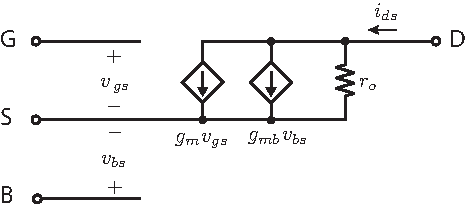
\includegraphics[scale=1.15]{mos4term_dc_gmb}}
\subcaptionbox{\label{fig:mos4term_ac_gmb}}{
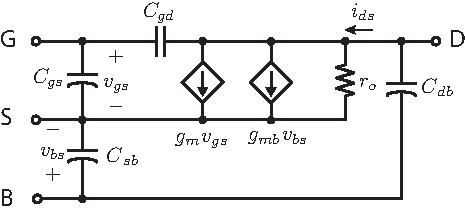
\includegraphics[scale=1.15]{mos4term_ac_gmb}}
\caption{The complete small-signal models for an $N$-type MOSFET with (a) no capacitors and with (b) capacitors.  The model without capacitors is useful for low frequency calculations.} 
\end{figure}
%%%%%%%%%%%%%%%%%%%%%%%%%%%%%%%%%%%%%%%%%%%%%%%%%%%%%%%%%%%%%%%%%%%%%%%%%%%%%%%%%%%%%%%%
%%%%%%%%%%%%%%%%%%%%%%%%%%%%%%%%%%%%%%%%%%%%%%%%%%%%%%%%%%%%%%%%%%%%%%%%%%%%%%%%%%%%%%%%
%                                   SECTION 10.4                                       %
%%%%%%%%%%%%%%%%%%%%%%%%%%%%%%%%%%%%%%%%%%%%%%%%%%%%%%%%%%%%%%%%%%%%%%%%%%%%%%%%%%%%%%%%
%%%%%%%%%%%%%%%%%%%%%%%%%%%%%%%%%%%%%%%%%%%%%%%%%%%%%%%%%%%%%%%%%%%%%%%%%%%%%%%%%%%%%%%%
\section{Complete Four Terminal MOS Small-Signal Model}
%%%%%%%%%%%%%%%%%%%%%%%%%%%%%%%%%%%%%%%%%%%%
%             SUBSECTION 10.4.1            %
%%%%%%%%%%%%%%%%%%%%%%%%%%%%%%%%%%%%%%%%%%%%
\subsection{Four-Terminal Small-Signal Model}
We now complete the small-signal model\index{MOSFET!small-signal!current with body bias} by noting that the drain-source current depends on $v_{gs}$ (transconductance), $v_{ds}$ (output resistance of device), and also on $v_{bs}$ (back-gate):
    \begin{align}
        \Aboxed{i_{ds} &= g_m\,v_{gs} + \left( \frac{1}{r_o} \right)v_{ds} + g_{mb}\,v_{bs}} &\textit{Small-signal current with body effect}
    \end{align}
This equation is captured by the equivalent circuit shown in \emph{Fig.~\ref{fig:mos4term_dc_gmb}}.  This model naturally shows the symmetry between the front-gate and the back-gate.  If we include all the capacitors as well, we arrive at \emph{Fig.~\ref{fig:mos4term_ac_gmb}}, the \textbf{complete small-signal model}\index{MOSFET!small-signal!complete model} for an $NMOS$ transistor.
%%%%%%%%%%%%%%%%%%%%%%%%%%%%%%%%%%%%%%%%%%%%
%             SUBSECTION 10.4.2            %
%%%%%%%%%%%%%%%%%%%%%%%%%%%%%%%%%%%%%%%%%%%%
\subsection{Complete Small-Signal Model PMOS}
Using the same arguments, we can also conclude that a PMOS device is also described by a similar four-terminal small-signal equivalent circuit model, as shown in \emph{Fig.~\ref{fig:pmos4term_ac}}.
%%%%%%%%%%%%%%%%%%%%%%%%%%%%%%%%%%%%%%%%%%%%
%                 FIGURE                   %
%%%%%%%%%%%%%%%%%%%%%%%%%%%%%%%%%%%%%%%%%%%%
\begin{figure}[h]
\centering
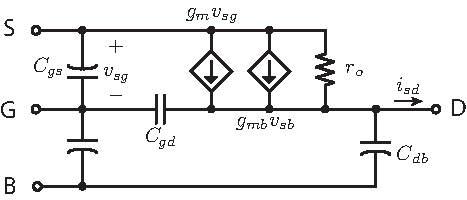
\includegraphics[scale=1.05]{pmos4term_ac}
\caption{The complete small-signal models for an $P$-type MOSFET.}
\label{fig:pmos4term_ac}
\end{figure}
%%%%%%%%%%%%%%%%%%%%%%%%%%%%%%%%%%%%%%%%%%%%
% \newpage
% %%%%%%%%%%%%%%%%%%%%%%%%%%%%%%%%%%%%%%%%%%%%%%%%%%%%%%%%%%%%%%%%%%%%%%%%%%%%%%%%%%%%%%%%
% %%%%%%%%%%%%%%%%%%%%%%%%%%%%%%%%%%%%%%%%%%%%%%%%%%%%%%%%%%%%%%%%%%%%%%%%%%%%%%%%%%%%%%%%
% %                                 SECTION 10.5                                         %
% %%%%%%%%%%%%%%%%%%%%%%%%%%%%%%%%%%%%%%%%%%%%%%%%%%%%%%%%%%%%%%%%%%%%%%%%%%%%%%%%%%%%%%%%
% %%%%%%%%%%%%%%%%%%%%%%%%%%%%%%%%%%%%%%%%%%%%%%%%%%%%%%%%%%%%%%%%%%%%%%%%%%%%%%%%%%%%%%%%
% \section{Chapter Summary}
% In this chapter we ...
